\title{Discrete Multivariate Modeling - Final Project}
\author{Ryan Spangler}
\date{\today}

\documentclass[11pt]{article}

\usepackage{commath}
\usepackage{graphicx}
\usepackage{listings}
\usepackage{amsfonts}

% python highlighting ----------
\usepackage{color}
\usepackage{listings}
\usepackage{textcomp}
\usepackage{setspace}
%\usepackage{palatino}

%\doublespacing

\setcounter{secnumdepth}{0}

\begin{document}
\maketitle

\section{Outline}

For my data I took a simulation I had previously written of two entities tracking each other in three dimensional space through time, and rendered out each position as either positive or negative for each axis.  I thought of this system as an ouroboros, with the head chasing its own tail.  This resulted in six variables, three for the position of each entity, each of cardinality 2 (positive or negative).  As it was a simulation I was able to generate several thousand points, and the simulation was nondeterministic enough that there is a complex (but strong!) relationship between the positions of the two entities.  This binning has the effect of detecting which of the eight octant volumes around origin each entity was in at any particular moment in the history of the simulation.  I took a periodic sampling of moments through time to compensate for the fact that the entities move continuously through space so that at any particular moment the entity is most likely in the same octant is was in the exact moment before.  

The data relationship in this case reads AxAyAzBxByBz (x, y and z for both entity A and entity B).  A snapshot of one run from the simulation is pictured below:

\begin{center}
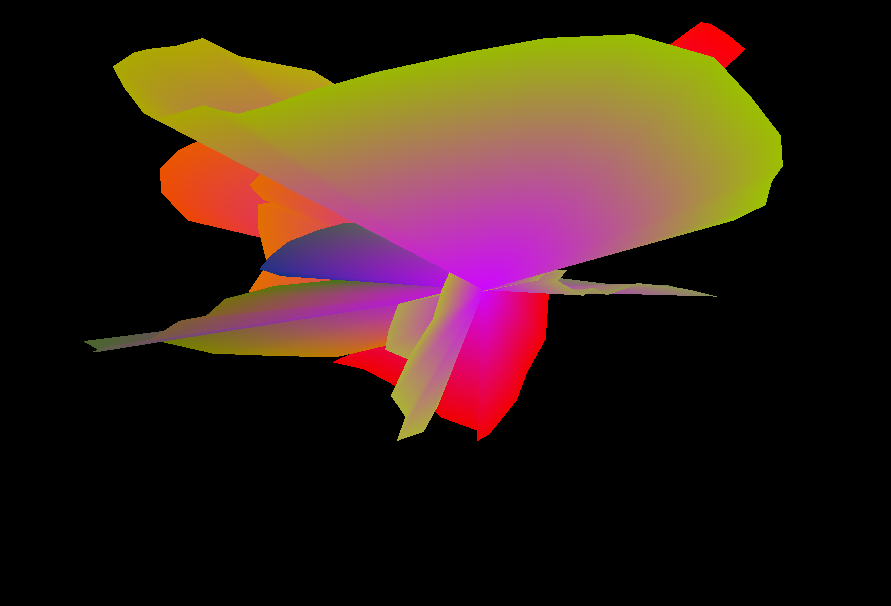
\includegraphics[scale=0.4]{ouroboros.png}
\end{center}

\section{Results}

My first run was an exploratory search of the space from the top down.  I had no dependent variables so my system is neutral, which defaults from the top and I saw no immediate reason to change this.  Here is a snippet from the results (with slight formatting):

\begin{verbatim}
MODEL,   Level,   H,   dDF,   dLR,   Alpha,   Inf,   dAIC,   dBIC
AxAyAzBxByBz, 0,5.7705, 0,  0.0000,1.0000,1.00000000, -0.0000, -0.0000
AxAyAzByBz:AxAzBxByBz, 1,5.7719,16, 17.6630,0.3436,0.99367081, 14.3370,127.7098
AxAyBxByBz:AyAzBxByBz, 1,5.7721,16, 20.2211,0.2099,0.99275415, 11.7789,125.1517
AxAyAzBxBz:AyAzBxByBz, 1,5.7724,16, 24.1783,0.0855,0.99133616,7.8217,121.1944
AxAyBxByBz:AyAzByBz, 2,5.7730,24, 31.6066,0.1368,0.98867439, 16.3934,186.4526
AxAyBxBy:AyAzBxByBz, 2,5.7737,24, 39.1076,0.0267,0.98598654,8.8924,178.9516
AxAyByBz:AxAzBxByBz, 2,5.7737,24, 39.5556,0.0239,0.98582600,8.4444,178.5035
AxAyBxBy:AxAyByBz:AyAzByBz, 3,5.7740,32,43.3084,0.0875,0.98448126, 20.6916,247.4371
AxAyByBz:AxAzBxBz:AxBxByBz, 3,5.7742,32,45.1272,0.0619,0.98382953, 18.8728,245.6183
AxAyByBz:AxBxByBz:AyAzByBz, 3,5.7743,32,46.3656,0.0484,0.98338577, 17.6344,244.3799
AxAyByBz:AxBxBy:AyAzByBz, 4,5.7746,36,50.3383,0.0568,0.98196223, 21.6617,276.7504
AxAyBy:AxAzBxBz:AxBxByBz, 4,5.7749,36,53.7497,0.0289,0.98073982, 18.2503,273.3390
AxAyByBz:AxBxByBz:AzBxBz, 4,5.7753,36,59.6713,0.0078,0.97861793, 12.3287,267.4174
AxAyByBz:AxBxByBz:AzBz, 5,5.7758,38,65.3374,0.0037,0.97658757, 10.6626,279.9229
AxAyBy:AxAzBxBz:AxBxBy, 5,5.7759,40,66.1846,0.0056,0.97628399, 13.8154,297.2473
AxAyBy:AxBxBy:AyAzByBz, 5,5.7759,40,66.9172,0.0047,0.97602147, 13.0828,296.5146
AxAyByBz:AxBxBy:AzBz, 6,5.7761,42,69.3101,0.0049,0.97516403, 14.6899,312.2934
AxAyBy:AxBxByBz:AzBz, 6,5.7765,42,73.9599,0.0016,0.97349787, 10.0401,307.6436
AxAyBy:AxAyBz:AxBxBy:AzBz, 7,5.7768,46,77.0560,0.0027,0.97238844, 14.9440,340.8907
AxAyBy:AxBxBy:AxByBz:AzBz, 7,5.7768,46,77.9326,0.0022,0.97207432, 14.0674,340.0141
AxAyBy:AxBxBy:AyAzBy:AyAzBz, 6,5.7770,44,80.4725,0.0006,0.97116421,7.5275,319.3026
AxAyBy:AxBxBy:AyAzBz, 7,5.7774,46,5.3020,0.0003,0.96943363,6.6980,332.6446
\end{verbatim}

My results saw no great change in uncertainty, though the degrees of freedom dropped dramatically.  The likelihood ratio, or error, increased monotonically as the models got simpler, which is not surprising.  Its delta was large enough to be significant.  Alpha dropped quickly, remaining at 0.34 and 0.20 for the next two simpler models down from the data, AxAyAzByBz:AxAzBxByBz and AxAyBxByBz:AyAzBxByBz, before dropping below 0.01 for everything after AxAyByBz:AxBxByBz:AzBxBz (the 13th model).  The generally low alpha means that the models do effectively simplify the data, as the probability that you were wrong to reject the null is low (the null here being that the model is the same as the data).  

AIC and BIC were more or less predictable, decreasing and increasing respectively in a mostly monotonic manner.  One notable contender was the model AxAyByBz:AxBxBy:AyAzByBz, which was simplified enough to make its high dAIC attractive.  This model I then used as the basis for a more focused search.

Searching down from AxAyByBz:AxBxBy:AyAzByBz yielded results which were uniformly extreme, all with dLR of over 2700.  Nothing was being gained here.  So I searched up from this model and discovered the same thing.  Possibly this was because I was searching in the space of all possible models, rather than just models without loops.

Later, when trying out a search from the bottom up, I received the following error from Occam!

\begin{verbatim}
Searching levels:
1 :ERROR: upward loopless search not implemented for neutral systems.
\end{verbatim}

Is it possible for Occam to ever implement all possible features and therefore be complete?  But I think we know the answer to that, and I take this message to be a poetic statement of the fundamental incompleteness of all human creations.

\section{Discussion}

In retrospect I realize that this data has more of a temporal relationship, whereas the positions of the two points in relation to one another at any particular moment shows less relationship.  The head follows the tail, so the position is related through a delay, but it could be coming from any octant to reach wherever the tail is now, so there is no direct relationship between where the head is and where the tail is at that time.  And really why should there be?  The model reflects the constraints, and I imposed no constraints on where in space the entities could go.  So there should be no relationship and in a way I was testing the null relation, where really the variables are mostly independent.  Finding interesting data turns out to be the hard part of this project, not using Occam to analyze it.  Occam needs a worthy dataset to work its magic, a dataset rich in hidden relationships.  This was not that set.  Still, I felt I got a feel for how to use Occam should I come across this worthy dataset of which I postulate, yet have not seen.

\end{document}  

